\documentclass[10pt]{article}
\usepackage[letterpaper,top=2.5cm,bottom=2.5cm,left=2.5cm,right=2.5cm]{geometry}
\usepackage{amsmath,amssymb}
\usepackage{graphicx}
\usepackage[colorlinks=true, allcolors=blue]{hyperref}
\usepackage[table,xcdraw]{xcolor}
\usepackage{float}
\usepackage{multirow}
\usepackage{caption}
\usepackage{subcaption}
\usepackage{tcolorbox}
\usepackage{booktabs}
\usepackage{subfiles}
\usepackage{import}
\usepackage{adjustbox}

\definecolor{captionblue}{rgb}{0.0, 0.0, 0.3}
\captionsetup{font={small,color=captionblue},labelfont={small,color=captionblue}}

\begin{document}

\title{Continuous Footstep Optimization for Quadruped Robots via
Projected Gradient Ascent}
\author{Your Name}
\date{}
\maketitle

\begin{abstract}
  Quadruped locomotion in unstructured environments remains a
  significant challenge. This paper proposes a novel method for
  generating non-gaited, dynamic footstep plans using GaitNet, which
  evaluates and selects the most appropriate actions. By directly
  exploring the output space through projected gradient ascent,
  GaitNet optimizes spatial footstep coordinates over its own reward
  surface. We formulate the problem with 4 parallel tracks and 4
  steps of projected gradient ascent per foot. Our system is
  evaluated on a physical Unitree Go1 robot navigating complex
  terrain, demonstrating improvements over state-of-the-art model
  predictive control baselines.
\end{abstract}

\section{Motivation and Vision}
\label{sec:introduction-motivation-and-vision}

Legged robots hold significant promise for enabling mobility in
environments that are inaccessible to wheeled and tracked systems.
Their ability to traverse uneven, unstructured, and unpredictable
terrains\textemdash such as disaster zones, staircases, dense
vegetation, and rocky landscapes\textemdash positions them as key
enablers for future exploration, inspection, and rescue missions.

Realizing this potential requires a robot to continuously and
intelligently decide where and when to place its feet\textemdash a
process known as \textit{contact planning}. Unlike periodic gait
patterns suitable for flat or predictable surfaces, real-world
locomotion often demands dynamic, acyclic, and adaptive footstep
sequences. Even minor errors in contact selection can lead to
instability or failure, whereas well-chosen footholds enable
efficient, agile, and robust movement.

The generation of such contact plans in real time remains a
formidable challenge. It requires the system to perceive its
surroundings, anticipate the outcomes of possible actions, and select
feasible contact points within tight temporal constraints. Existing
methods often fall into one of three categories, fully using
traditional control\textemdash model predictive controllers, PD
controllers, optimization\textemdash using neural networks, or a mix
of the two: hybrid methods. These three methods offer different trade
offs between deliberative, computationally intensive planning and
fast, reactive control that lacks stability or generalization.

The vision of this research is to develop a hybrid control
architecture that optimizes these trade offs. Specifically, this work
aims to design a system capable of producing non-gaited, dynamic
footstep plans that retain both the responsiveness of learning-based
approaches and the reliability of model-based control. The objective
is to provide quadruped robots with the decision-making agility
necessary for navigating complex terrains while maintaining the
stability and robustness demanded by real-world operation.

Through this approach, the thesis seeks to contribute toward a new
class of hybrid locomotion frameworks that enable real-time,
adaptive, and physically consistent quadruped motion\textemdash
closing the gap between high-level perception and low-level control
in legged robotics.
\section{Research Gap}
\label{sec:introduction-research-gap}

Quadruped control pipelines can be categorized into several
approaches, many of which can be broadly classified as traditional,
neural network-based, or hybrid methods.

Traditional approaches typically rely on model predictive control
(MPC) frameworks for motion optimization, supported by lower-level
controllers to track desired trajectories
\cite{Kim2019highly-dynamic}. Many aspects of quadruped
locomotion\textemdash such as joint torques and ground reaction
forces\textemdash are smooth and well-suited to continuous
optimization techniques
\cite{Wensing2022Nov}. However, these methods become less tractable
when discrete contact states are introduced into the optimization
problem \cite{Geisert2019contact-planning}. To manage this
complexity, most implementations either assume pre-defined gait
sequences \cite{Chai2022survey, Fan2024survey} or encode discrete
contact decisions within larger optimization structures
\cite{winkler_gait_2018}. While effective in structured environments,
these strategies constrain the robot's ability to exploit the full
versatility of legged locomotion by reducing the dimensionality of
expressable states for the system.

Neural network-based methods have emerged as an alternative,
particularly with advances in deep reinforcement learning. These
approaches often replace the MPC component of traditional control
pipelines, learning to directly map observed states to joint torques
or motion commands \cite{Gurram2024survey}. In doing so, they
inherently address the mixed-integer nature of contact planning,
allowing the network to learn both continuous and discrete aspects of
locomotion simultaneously \cite{Wensing2022Nov}. Despite their
flexibility, such methods generally lack formal guarantees of
stability, require substantial training data, and often struggle to
generalize beyond their training distribution \cite{Gurram2024survey}.

Hybrid approaches, which integrate learning-based modules within
model-based control frameworks, have recently gained attention as a
potential middle ground. In these systems, neural networks are
typically employed to solve specific subproblems\textemdash such as
dynamically switching between fixed gaits or greedily selecting
individual footholds\textemdash while the overall motion execution
remains governed by a traditional controller \cite{Bao2024survey,
Wang2022Oct}. This division of responsibilities enables learning to
focus on the non-smooth or combinatorial components of locomotion,
while preserving the interpretability, safety, and robustness
inherent to model-based systems.

Looking at how each of these categories handles the contact planning
problem, hybrid control schemes have demonstrated promise, the
challenge of contact and footstep planning continues to limit their
performance. Traditional optimization-based planners struggle with
the discrete nature of contact transitions, resulting in high
computational costs that preclude real-time operation
\cite{winkler_gait_2018}. Alternatively, many rely on pre-specified
gait patterns \cite{xie_glide_2023, grandia_perceptive_2022,
lee_learning_2020, villarreal_fast_2019}, constraining adaptability
to irregular or unpredictable terrain. Even more advanced approaches,
such as Monte Carlo Tree Search (MCTS)-based planners, have achieved
impressive dynamic behaviors but remain computationally demanding
\cite{amatucci_monte_2022, taouil_non-gaited_2024}. Finally, end to end
learning methods solve these problems implicitly, but at the cost of
control theory guarantees and interpretability.

Despite recent progress, a clear research gap remains. Current hybrid
methods do not yet achieve the balance between adaptability and
stability that would enable fully dynamic, acyclic locomotion in
complex environments. In particular, there is a lack of systems that
can match the contact planning agility of neural network-based
approaches while retaining the formal guarantees and reliability of
traditional control frameworks \cite{Meng2023Mar, Wensing2022Nov}.
Recent supervised learning estimators have
demonstrated the potential of machine learning for footstep evaluation;
however, their design\textemdash often restricted to single-leg motions with
fixed timing\textemdash still falls short of the dynamic, non-gaited
behaviors exhibited by end-to-end learning systems.

This motivates a central research question:

\begin{quote}
  \textbf{Can a hybrid control pipeline, which integrates a greedy,
    neural-network-based planner with a traditional model-based
    controller, generate dynamic, acyclic gaits for robust quadruped
  locomotion in challenging environments?}
\end{quote}
\section{Approach}
\label{sec:introduction-approach}

The proposed approach bypasses traditional discrete sampling or
candidate generation networks entirely. Instead, a novel
single-network architecture, \textit{GaitNet}, is used to evaluate
and select the most appropriate action at each time step. By directly
exploring the output space through projected gradient ascent, GaitNet
optimizes spatial footstep coordinates directly over its own reward
surface. By integrating this continuous optimization planner within a
traditional model-based control framework, we harness the advantages
of rapid learning-based evaluation and robust model-based
stabilization, yielding an adaptable quadruped locomotion system.


\section{Methodology}
\label{sec:methodology}
\subsection{System Overview}
\label{subsec:methodology-system-overview}

This work presents a control framework for quadruped robots capable of generating dynamic, acyclic gaits in challenging environments. The framework employs a hierarchical architecture that processes robot state and terrain data to produce footstep commands for the robot controller. 

The first stage of the framework receives user input $\mathbf{v^{usr}}$ alongside the tracking robot state $\mathbf{x_g}$ into the gait generation network (\textit{GaitNet}). GaitNet acts as an evaluative surface, performing continuous optimization over the physical workspace using projected gradient ascent. Rather than extracting from a discrete sample grid, GaitNet iteratively ranks these continuous spatial variables to yield an optimal footstep action $\mathbf{f_a}$. This optimal action is then passed downstream to a traditional MIT Mini-Cheetah Controller \cite{di_mini_cheetah_2020}. This hierarchical design ensures strict control over potential actions and prevents violations of physical constraints.

\begin{figure}[H]
  \centering
  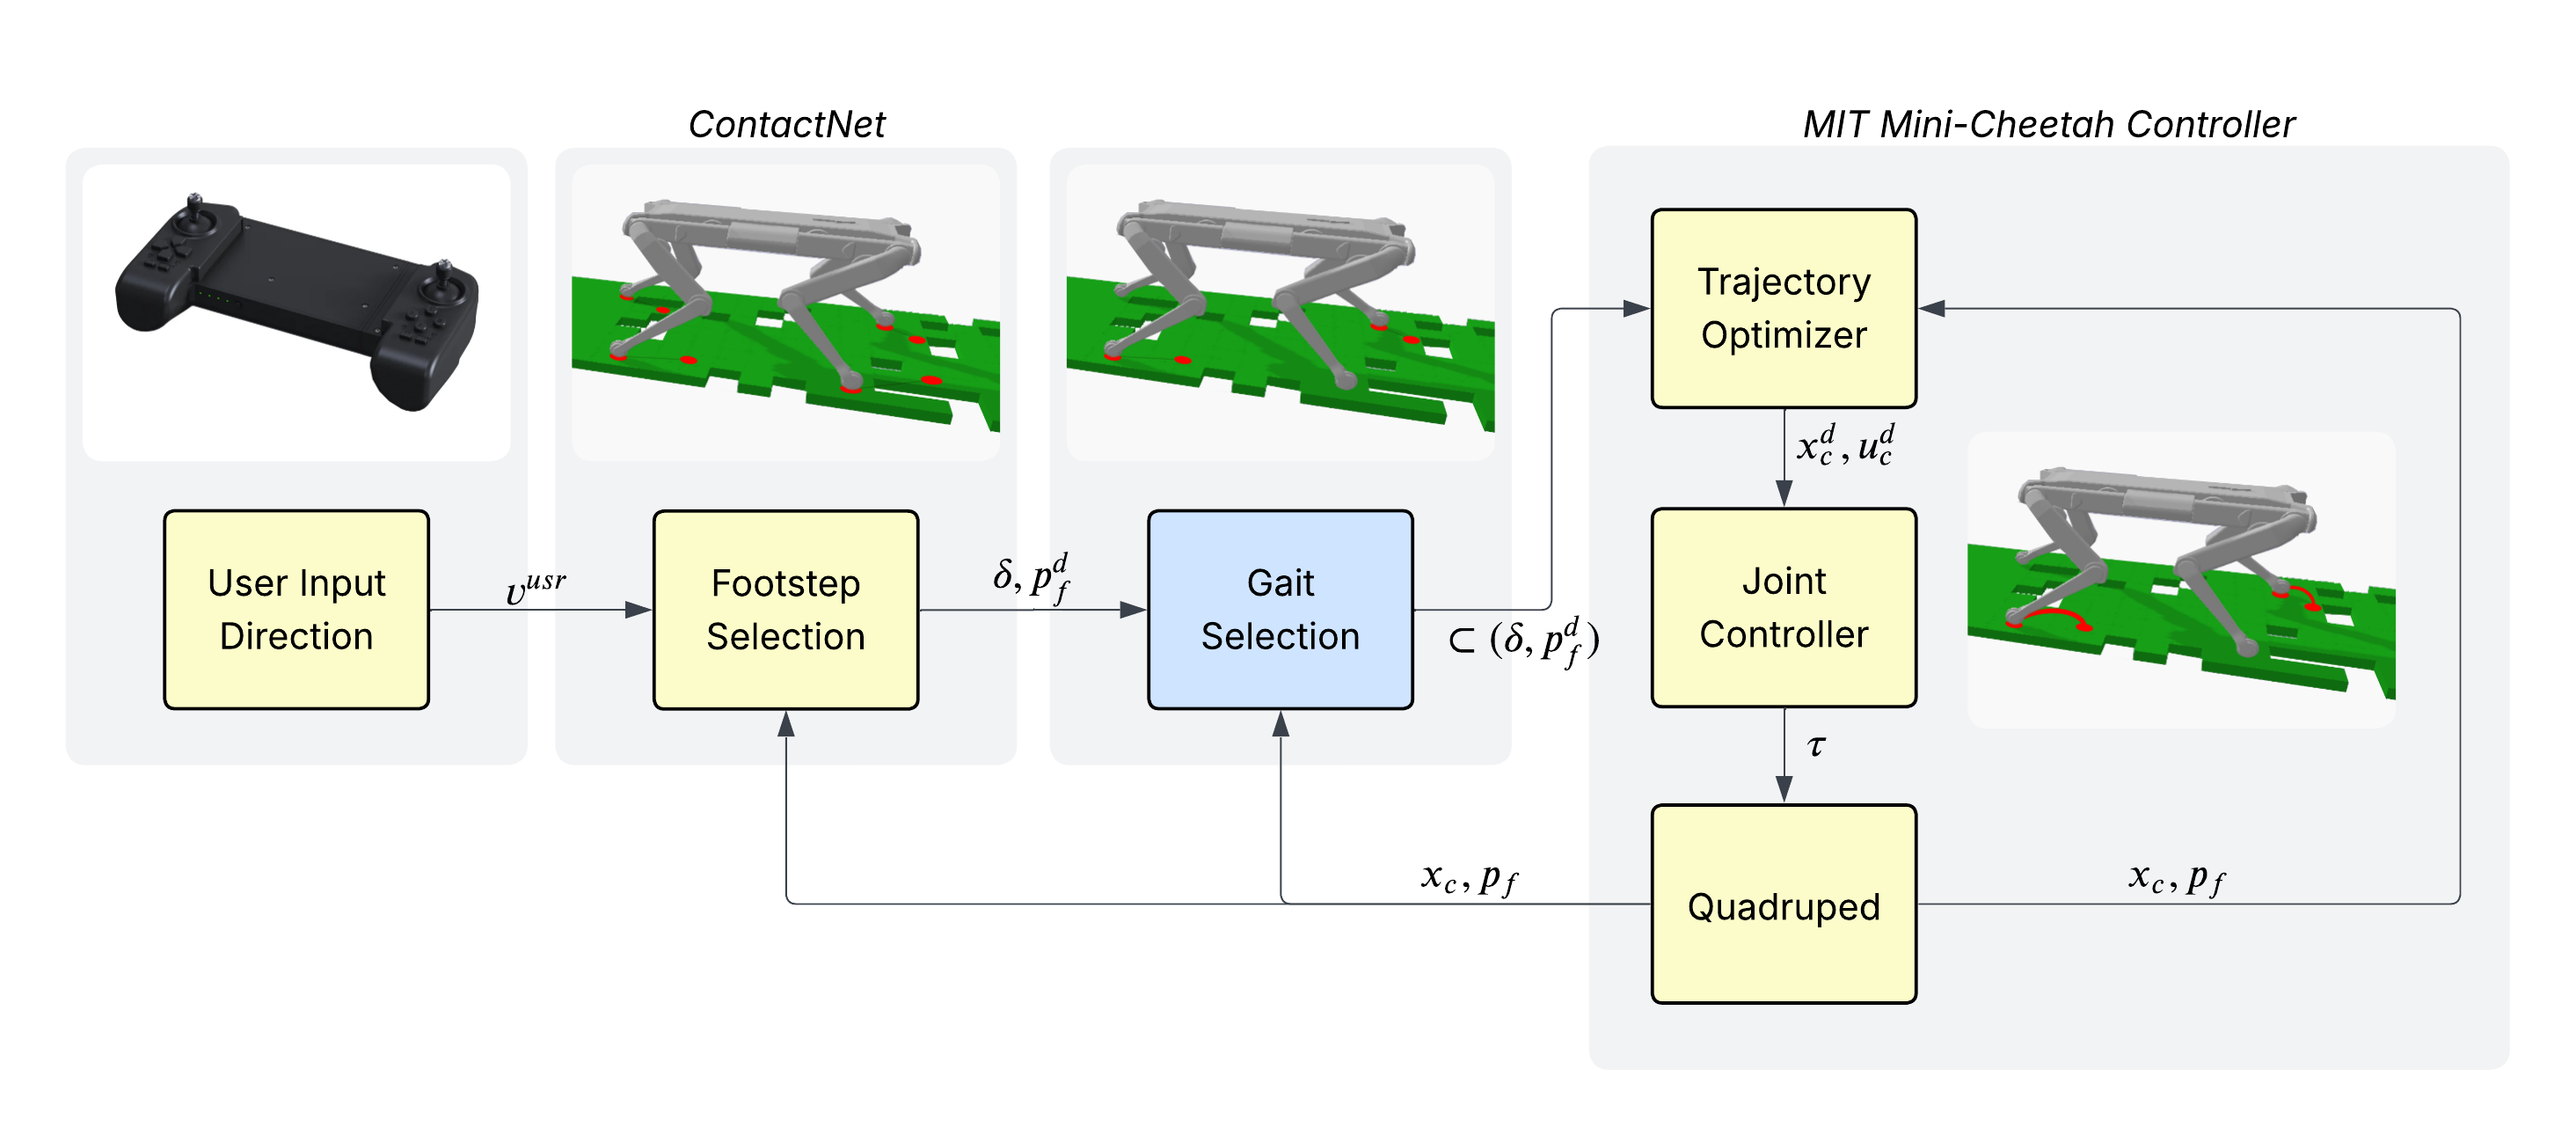
\includegraphics[width=0.7\linewidth]{images/diagrams/control-system.png}
  \caption{Block diagram of the proposed framework. The user defines an input direction $\mathbf{v^{usr}}$, which GaitNet uses along with the robot state $\mathbf{x_g}$ and current foot positions $\mathbf{p_f}$ to evaluate candidate footsteps. GaitNet utilizes a continuous projected gradient ascent optimization strategy to generate optimal step actions $\mathbf{f_a}$ for the controller.}
  \label{fig:diagram-control-system}
\end{figure}

\subsection{GaitNet Architecture}
\label{subsec:methodology-gaitnet-architecture}

GaitNet is a single-network architecture composed of a state encoder, footstep encoder, shared trunk, and two task-specific output heads (one predicting logit rewards and another predicting swing duration). It ranks footstep candidates based on the one-hot encoded leg index $\mathbf{f_c}^{\prime}$ and the state $\mathbf{x_g}$, which tracks the current base position $\mathbf{p}_{b,xy}$ and rotation $\mathbf{r}_{w,z}$, body velocities $\mathbf{v}_b$ and $\mathbf{\omega}_b$, current foot positions $\mathbf{u}$, gravity $\mathbf{g}$, and contact state $\mathbf{c}$. Both the continuous spatial coordinates and a fixed ``no-action'' embedding are evaluated simultaneously.

\subsection{Projected Gradient Ascent Optimization}
\label{subsec:methodology-gaitnet-gradient-ascent}

Footstep selection is formulated as a continuous optimization problem over the spatial coordinates. GaitNet’s predicted reward logit acts as a differentiable objective function maximized via projected gradient ascent.

For each foot, $N=4$ random initial spatial samples are drawn uniformly from the reachable kinodynamic workspace. The algorithm performs 4 parallel steps of projected gradient ascent to maximize the GaitNet evaluation logit. After each gradient update step, spatial coordinates are projected back to the nearest valid configuration within the reachable stepping continuous space (c-space). This projection acts as a hard constraint that forces foot locations to avoid un-steppable obstacles (such as gaps or rough geometry) while preserving maximal reward.

Concurrently, a fixed ``no-action'' embedding is evaluated. Once the 4 projection and ascent steps finish, the candidate yielding the highest reward logit across all $4 \times 4$ tracks is compared to the ``no-action'' logit. The action with the maximum reward is output as $\mathbf{f_a}$ and deployed to the inner controller at control frequencies.

\subsection{Network Training}
\label{subsec:methodology-gaitnet-training}

GaitNet is trained using Proximal Policy Optimization (PPO) \cite{Schulman_proximal_2017} acting directly as the policy network, with a structurally similar critic network. Given the dual discrete-continuous nature of the task, the logits parameterized a categorical distribution over tracks, while the duration output constitutes a normal distribution with fixed standard deviation. The continuous spatial coordinates are trained synchronously under the PPO agent formulation.


\section{Experimental Results}
\label{sec:results}
\subsection{Physical Robot Experiments and Baseline Comparison}
\label{subsec:results-baseline-comparison}

To evaluate GaitNet's continuous optimization strategy in
unstructured real-world scenarios, a baseline method is established
utilizing the \textit{Legged Perceptive Stack} \cite{leggedcontrol}.
This state-of-the-art framework employs Nonlinear Model Predictive
Control (NMPC) and Whole-Body Control (WBC) based on OCS2.

A custom physical test environment was constructed mirroring our
simulation benchmark parameters
(\autoref{fig:figure-test-environment}). Hardware experiments were
conducted on a Unitree Go1 quadruped navigating narrow strips of
ground interspersed with gaps. We characterize terrain difficulty
metrics as the percentage of unsteppable terrain (ranging from $0\%$
to $40\%$ gap densities).

We systematically evaluate success rate (completing traversal without
falling), total steps taken, and overall traversal time of the
following methods:
\begin{enumerate}
  \item \textbf{Legged Perceptive Stack:} The state-of-the-art model
    predictive control baseline \cite{leggedcontrol}.
  \item \textbf{GaitNet-Single:} An ablation of GaitNet restricted to
    only one leg in swing phase at any given time.
  \item \textbf{GaitNet-Trot:} An ablation of GaitNet restricted to
    only opposing legs in swing concurrently.
  \item \textbf{GaitNet (Full):} Our proposed unlimited acyclic
    footprint generation model.
\end{enumerate}

\begin{figure}[H]
  \centering
  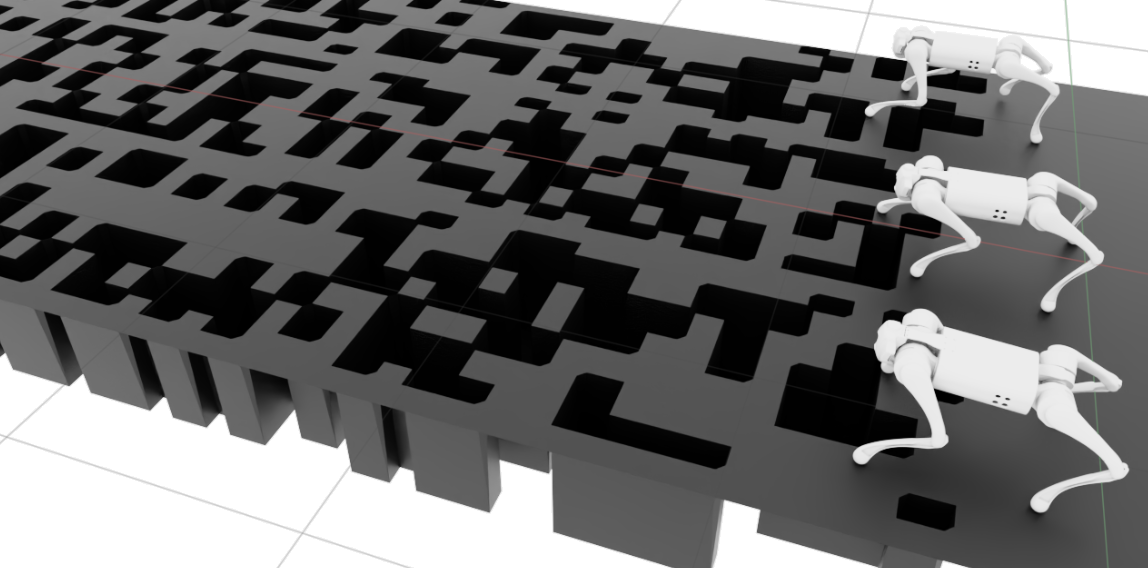
\includegraphics[width=0.8\textwidth]{images/figures/test-environment.png}
  \caption{Unitree Go1 navigating the physical test environment used
    for baseline comparison. The terrain consists of narrow strips
  mapping to varying terrain difficulties (percentage of unsteppable terrain).}
  \label{fig:figure-test-environment}
\end{figure}

GaitNet's unconstrained performance relative to the Legged Perceptive
Stack and fixed-gait ablations reveals a clear advantage in dynamic,
acyclic spatial optimization. The system coordinates multi-leg
motions and adapts continuous spatial timing to minimize total steps
while avoiding invalid terrain. This improvement is particularly
pronounced at higher terrain difficulties ($30$-$40\%$ gap
densities), where restrictive trot strategies inherently clash with
unstructured valid footprints.

\begin{table}[H]
  \centering
  \caption{Placeholder: Real-World Metrics on Unitree Go1}
  \begin{tabular}{lccc}
    \toprule
    \textbf{Method} & \textbf{Success Rate} & \textbf{Avg. Traversal
    Time [s]} & \textbf{Avg. Steps Taken} \\
    \midrule
    Legged Perceptive Stack & XX\% & XX.X & XXX \\
    GaitNet-Single & XX\% & XX.X & XXX \\
    GaitNet-Trot & XX\% & XX.X & XXX \\
    \textbf{GaitNet (Full)} & \textbf{XX\%} & \textbf{XX.X} & \textbf{XXX} \\
    \bottomrule
  \end{tabular}
  \label{tab:hardware-metrics}
\end{table}

\subsection{Simulation Ablations}
\label{subsec:results-simulation-ablations}

In addition to physical trials, simulation ablations were conducted
to validate specific structural choices, notably the swing duration
penalty and action costs within GaitNet. We analyze performance on
similar unstructured tracks but over a more extensive $200$ episode benchmark.

An ablation assessing fixed uniform swing durations versus GaitNet's
dynamic network-predicted durations revealed that the addition of the
duration network head allowed the robot to effectively slow down its
stepping speed over sparse gaps as necessary to maintain equilibrium
while pushing faster transit on solid areas.

Similarly, an action cost penalty of $-0.05$ applied to any
non-no-action choice proved crucial to minimizing jittery or
inefficient consecutive sub-steps. Models evaluated without action
penalties consistently opted for inefficient high-frequency steps
compared to the clean traversal achieved by the penalized model.
GaitNet leverages these continuous penalty variables effectively to
prune excessive locomotion loops and stabilize the quadruped's
spatial gradients.


\section{Conclusion}
\label{sec:conclusion}
This work presented an integrated control framework capable of
generating dynamic, acyclic contact sequences by unifying
learning-driven evaluation via GaitNet with traditional model-driven
controllers. In contrast to discrete sampling schemas, evaluating
continuous candidate spaces through iterative projected gradient
ascent ensures maximal expected utility while projecting footsteps
out of un-steppable spaces.

Our method enables fully reactive, acyclic walking and trot behavior,
accommodating simultaneous swing phases when physically advantageous.
The real-world hardware deployment on the Unitree Go1 demonstrates
clear advantages in success rate across challenging gap-densities
compared to fixed-gait or predictive control baselines.

Future work will expand the action space to dynamic posture shifts
and whole-body optimization to tackle steeper terrain gradients
without manual scaling.


\bibliographystyle{ieeetr}
\bibliography{refs}

\end{document}
